\chapter{Betrag, Ungleichungen, Kreis}
\section{Betrag}
Autor: Marc Mittner

\noindent "Uberarbeitung: Christian Rutsch

\subsection{Definition}
F"ur eine reelle Zahl $x$ ist der Betrag definiert als: 

%\large
%$ | x | =  \left\{ ^{  x , x \geq 0}_{-x , x < 0} \right. $
$\vert x \vert = \left\{
\begin{array}{ccc}
x, && x \geq 0\\
-x,&&x < 0
\end{array}\right.$
%\normalsize

\subsection{Die Betragfunktion}
Graph der Betragfunktion $ f(x) = |x| $ ist:
\begin{itemize}
\item symmetrisch zur y-Achse 
\item $y \geq 0$ f"ur alle Werte $ x \in \mathbb{R} $.
\end{itemize}

\begin{center}
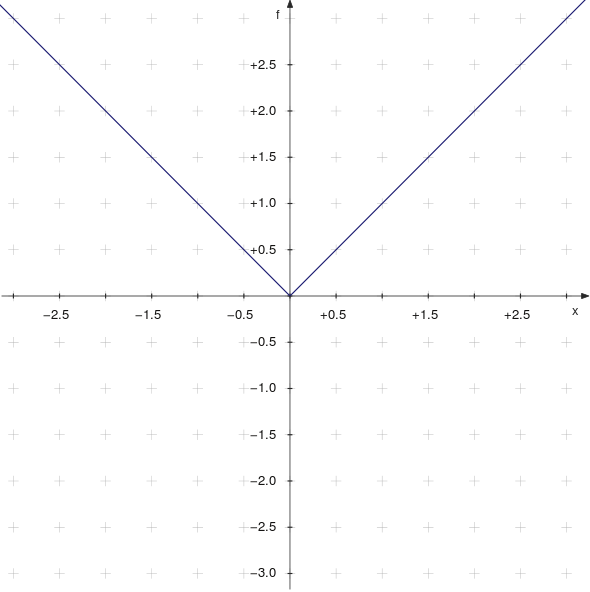
\includegraphics[scale=0.25]{img/betrag/betrag.png}
\end{center}

%\pagebreak
\subsection{Rechenregeln f"ur den Betrag}
\begin{enumerate}
\item $|-a|=|a|$
\item $|a|\geq0; |a|=0\Leftrightarrow a=0$
\item $|a\cdot b|=|a|\cdot |b|$
\item $|\frac{a}{b}|=\frac{|a|}{|b|}$ f"ur b$\neq0$
\item $|a^n|=|a|^n$ f"ur n$\in\mathbb{N}$
\item $|a+b|\leq|a|+|b|$ (sogenannte Dreiecksungleichung)
\end{enumerate}
\subsection{Beispiele}
Gleichungen mit Betr"agen werden durch Fallunterscheidung gel"ost.
\begin{enumerate}
 \item $ | x-1 | = 3 $

Fallunterscheidung

1.Fall:
\begin{align*}
  (x - 1) &= 3 \\
  x &= 4
\end{align*}

2. Fall:
\begin{align*}
-(x - 1) &= 3 \\
 x &= -2
\end{align*}



\item $(x + 3)^2 = 4   \rightarrow | x+3 | = 2$
   
Fallunterscheidung

1. Fall:
\begin{align*}
+(x + 3) &= 2 \\
\rightarrow x &= -1
\end{align*}
2. Fall:
\begin{align*}
-(x + 3) &= 2 \\
\rightarrow -x - 3 &= 2\\
 \rightarrow x &= -5
\end{align*}

\end{enumerate}

\subsection{Aufgaben}
L"osen Sie die folgenden Gleichungen: 
\begin{enumerate}
\item $|x| = 7$
\item $| x+5 | = 10$
\item $| 2x-3 | = 1$
\item $| 2x-4| = 6x+36$
\end{enumerate}
